% Charlotte Geiger - Manuel Lippert - Leonard Schatt
% Physikalisches Praktikum

% Teilaufgabe 6

\section{Kreiselkompass}
Bei einem rotierender Kreisel auf den keine Drehmomente wirken, behält der Drehimpuls seine Richtung bei, weswegen ein Kreisel als Kompass geeignet ist. Für eine kräftefreien Kreisel wird eine sogenannte \dq Cardano-Aufhängung\dq{} verwendet, welche verhindert, dass die Schwerkraft auf den Kreisel ein Drehmoment auswirken kann, was eine Drehimpulsänderung zur Folge hätte. In der Cardano Aufhängung wird dann der Kreisel möglichst reibungsfrei auf zwei sich im Schwerpunkt des Kreisels senkrecht schneidenen Achsen gelagert. Ein Kreiselkompass wird auch zur Navigation im Weltraum verwendet, was heutzutage schon in Satelliten und Sonden umgesetzt wird.
\begin{figure}[h]
    \centering
    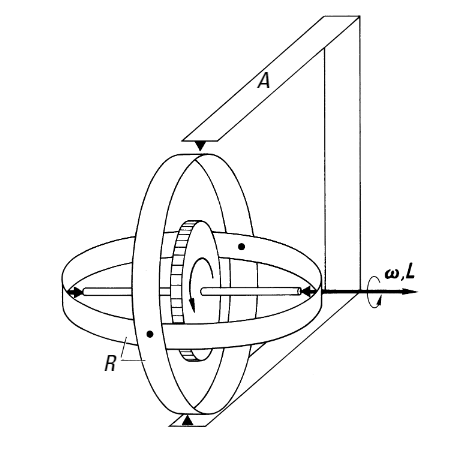
\includegraphics[width = 6cm]{Bilder/Kraeftefreie_Aufhaengung.PNG}
    \caption[Caption for LOF]{Kräftefreie Aufhängung eines Kreisels / Cardano-Aufhängung \footnotemark}
\end{figure}
\footnotetext[1]{Bergmann-Schäfer, Lehrbuch der Experimentalphysik Band 1, S.278}